% !TeX spellcheck = en_GB
% !TeX encoding = UTF-8 

\documentclass[14pt,a4paper]{extarticle}

\usepackage[english]{babel}
\usepackage[utf8]{inputenc}
\usepackage{setspace} 
\usepackage[a4paper,
			left=30mm,
			right=10mm,
			top=20mm,
			bottom=20mm]{geometry}
\usepackage{amsmath,amssymb,amsthm}
\usepackage{cite}
\usepackage{graphicx} 
\usepackage{subfigure,subcaption}
\usepackage{kprjHSE} 
\usepackage{tikz}
\usepackage{xcolor,tabularray}
\usepackage{wrapfig}
\usepackage{hyperref}
\hypersetup{
	colorlinks=true,
	linkcolor=black,
	citecolor=black,
	filecolor=black,      
	urlcolor=blue,
}

\usetikzlibrary{positioning}

\renewcommand{\labelenumii}{\arabic{enumi}.\arabic{enumii}}

\lstset{
	frame=single,
	basicstyle=\ttfamily,
	breaklines=true,
	tabsize=4
}

\LabWork
\title{Neural FCA}
\setcounter{MaxMatrixCols}{20}

\FirstAuthor{M.D.~Kirdin}
\FirstConsultant{A.~Tomat}
\SecondConsultant{M.~Zueva}
\discipline{Ordered Sets for Data Analysis}
\faculty{Faculty of Computer Science}
\chair{School of Data Analysis and Artificial Intelligence}
\chief{S.O.~Kuznetsov}
\workyear{2024}

\onehalfspacing

\begin{document}
	\maketitle
	
	\tableofcontents
	
	\begin{introduction}
		
		The overarching task of this homework is to implement a merger of machine learning and formal concept analysis. This is done by basing the neural network(NN) architecture on the covering relation (graph of the diagram) of a lattice coming from monotone Galois connections as proposed by Kuznetsov and his colleges \cite{NN_FCA}. The vertices of such NNs are related to sets of similar objects with similarity given by their common attributes, thus they are easily interpretable. The edges between vertices can be interpreted in terms of concept generality (bottom-up) or conditional probability (top-bottom). 
		
		You can find the source code for this homework at \url{https://github.com/succSeeded/NeuralFCA}.
		
	\end{introduction}
	
	\section{Model evaluation}
	\subsection{Problem statement}
	
	For this, a dataset has to be chosen, its data binarized using scaling (binarization) strategy of choice, and finally the target attribute defined. Then, a comparison between several standard classification methods and NN should be made by calculating performance metrics best suited for the dataset.
	
	\subsection{Model evaluation on the Employee Attrition dataset}
	
	The Employee Attrition dataset has 15K entries after dropping of all rows containing at least one empty value, hence it was decided to work only with a selection of 2400 randomly selected elements of this set.
	
	The NNs based on 4(minimal concept amount that covers all the training data) and 20 best-performing formal concepts with all the numerical features binarized using ordinal encoding with 3 nodes will serve as our baseline. Here the performance of each concept was measured as $f_1$-score of its extent used as a prediction. This produces architectures that can be seen on \figref{fig:4concepts} and \figref{fig:20concepts}. The results of baseline classification can be seen in the table A.1.
	
	\begin{figure}[h]
		\centering
		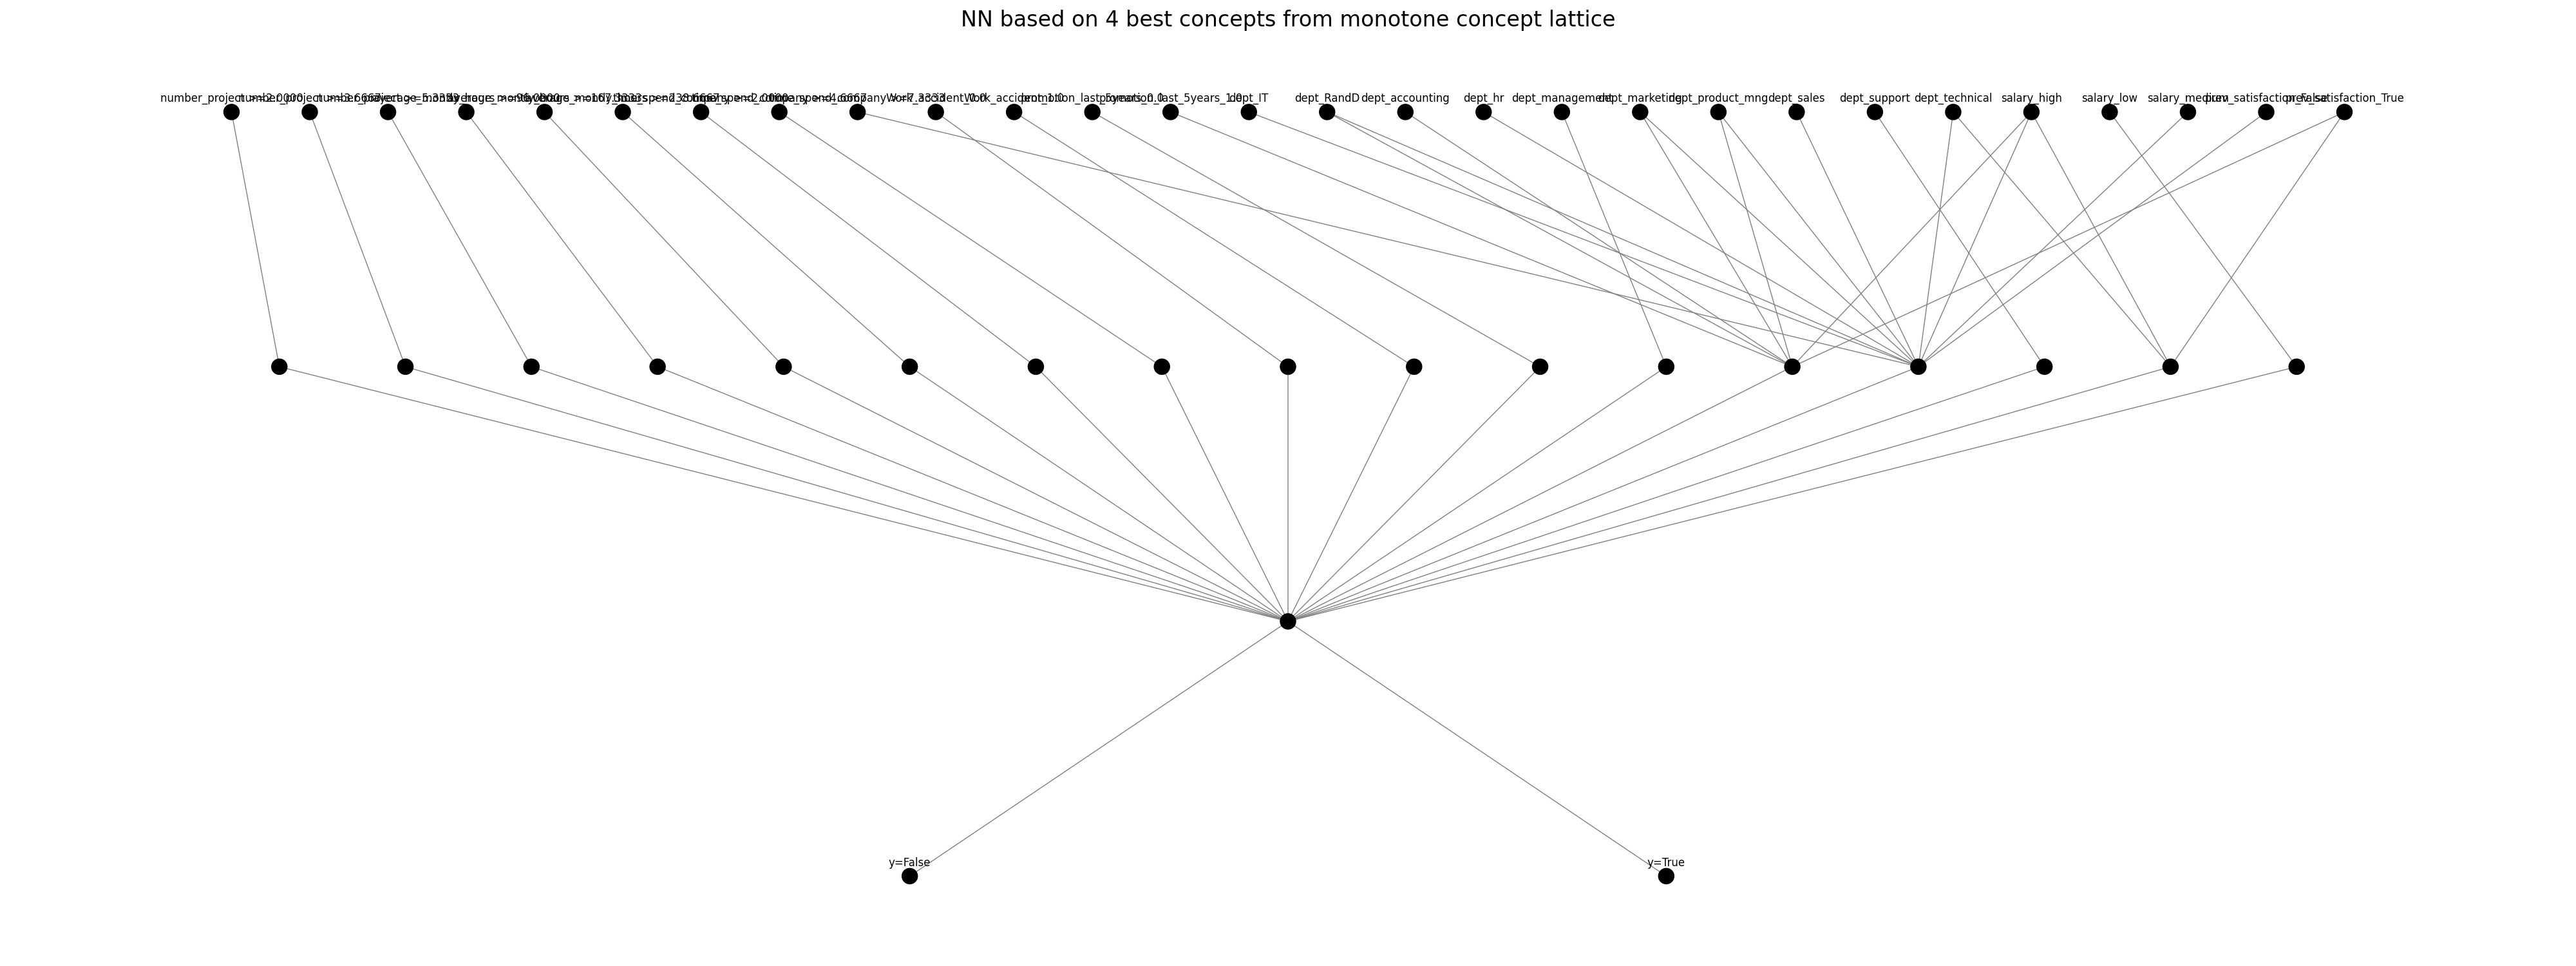
\includegraphics[width=\textwidth]{media/employees/NN_architecture_4concepts.png}
		\caption{NN architecture produced with the 4 best formal concepts(FCs)}
		\label{fig:4concepts}
	\end{figure}
	
	\newpage
	
	\begin{figure}[h]
		\centering
		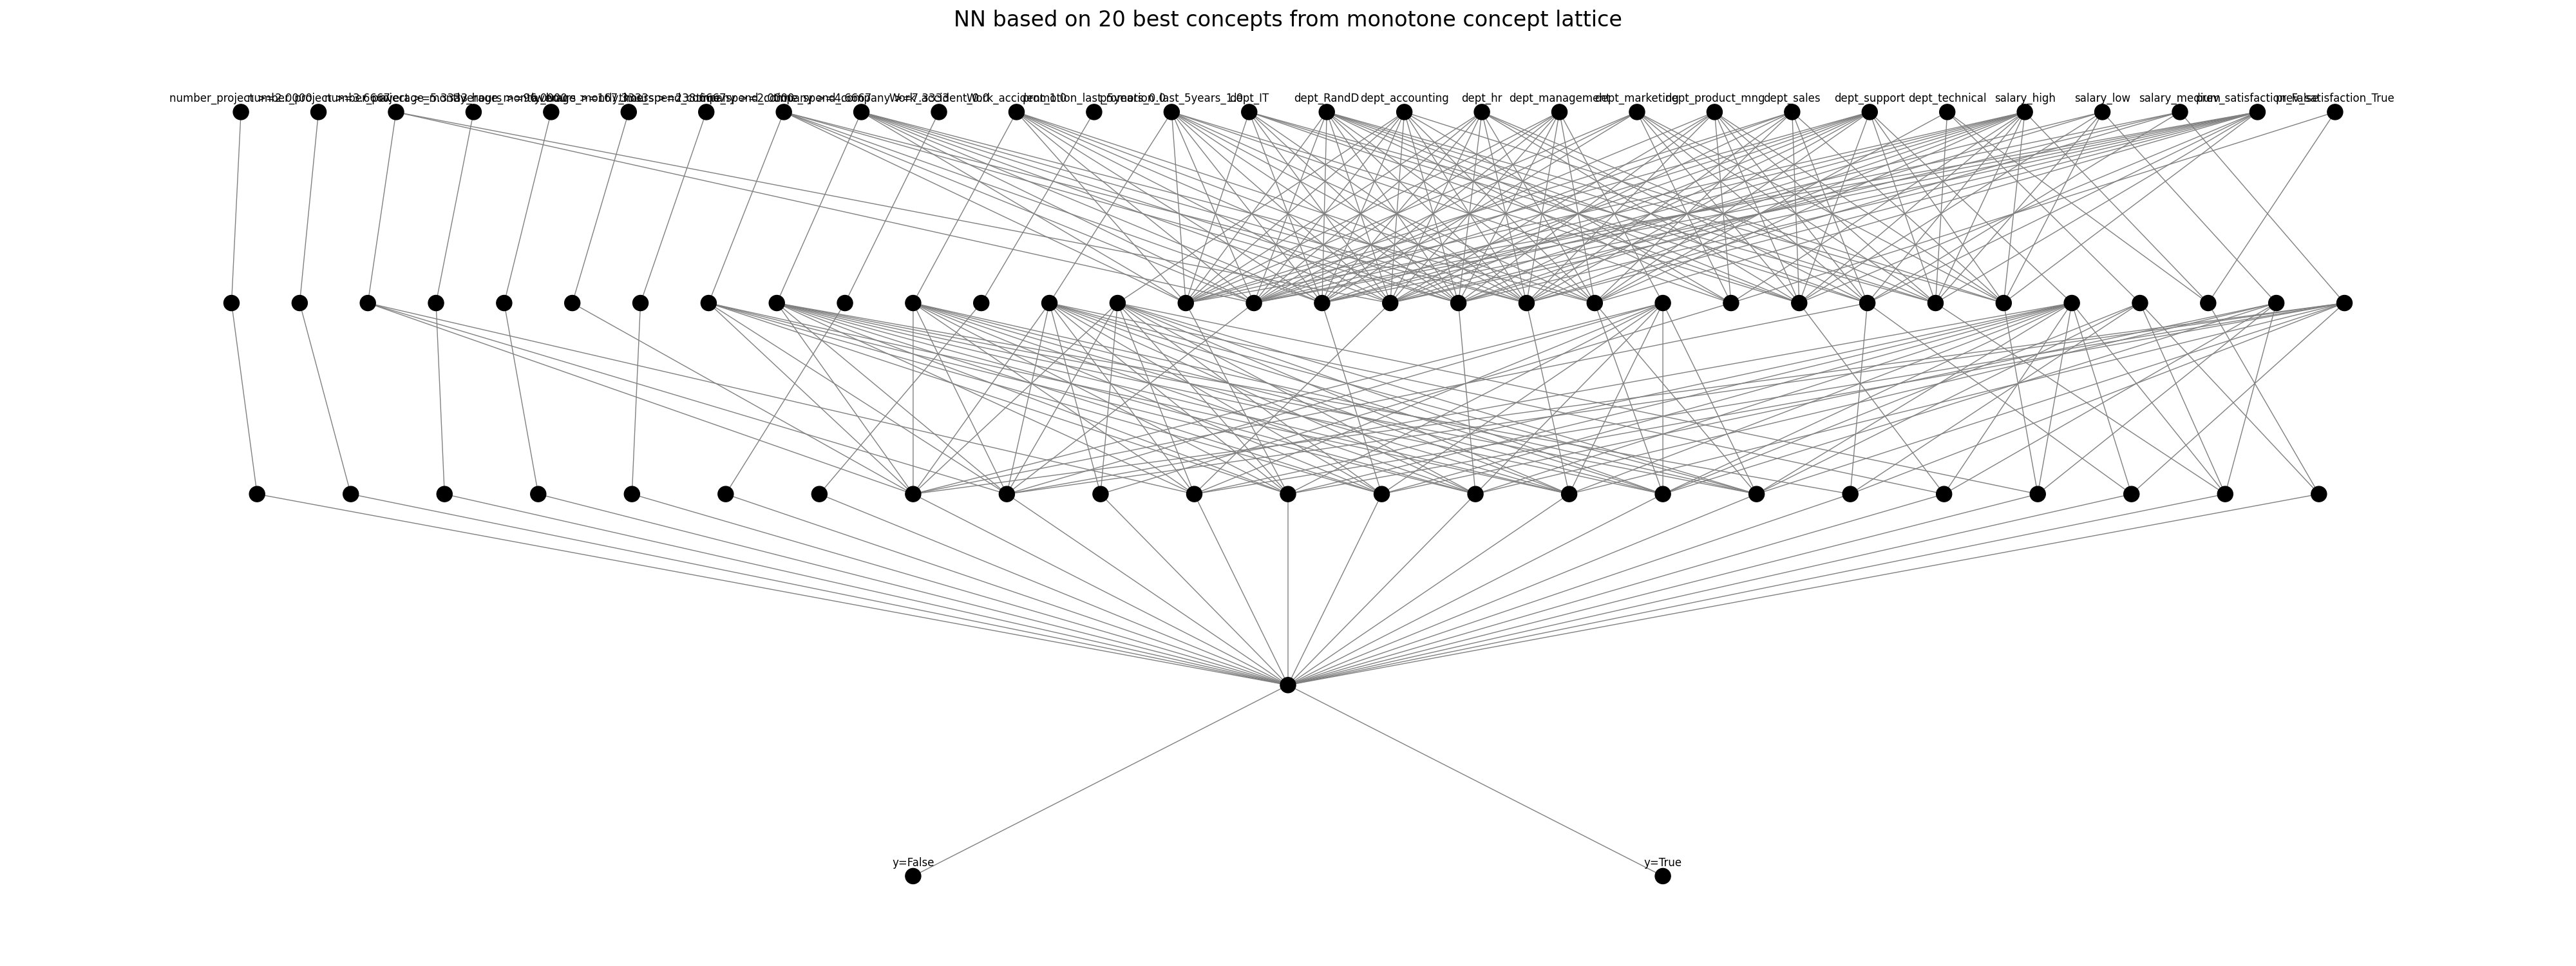
\includegraphics[width=\textwidth]{media/employees/NN_architecture_20concepts.png}
		\caption{NN architecture produced with the 20 best formal concepts(FCs)}
		\label{fig:20concepts}
	\end{figure}
	
	Another binarization type of interest is interordinal encoding. With double the amount of nodes it produces architectures seen on \figref{fig:4concepts-inter} and \figref{fig:20concepts-inter}, its performance metrics are recorded in the table A.2. 
	
	\begin{figure}[h]
		\centering
		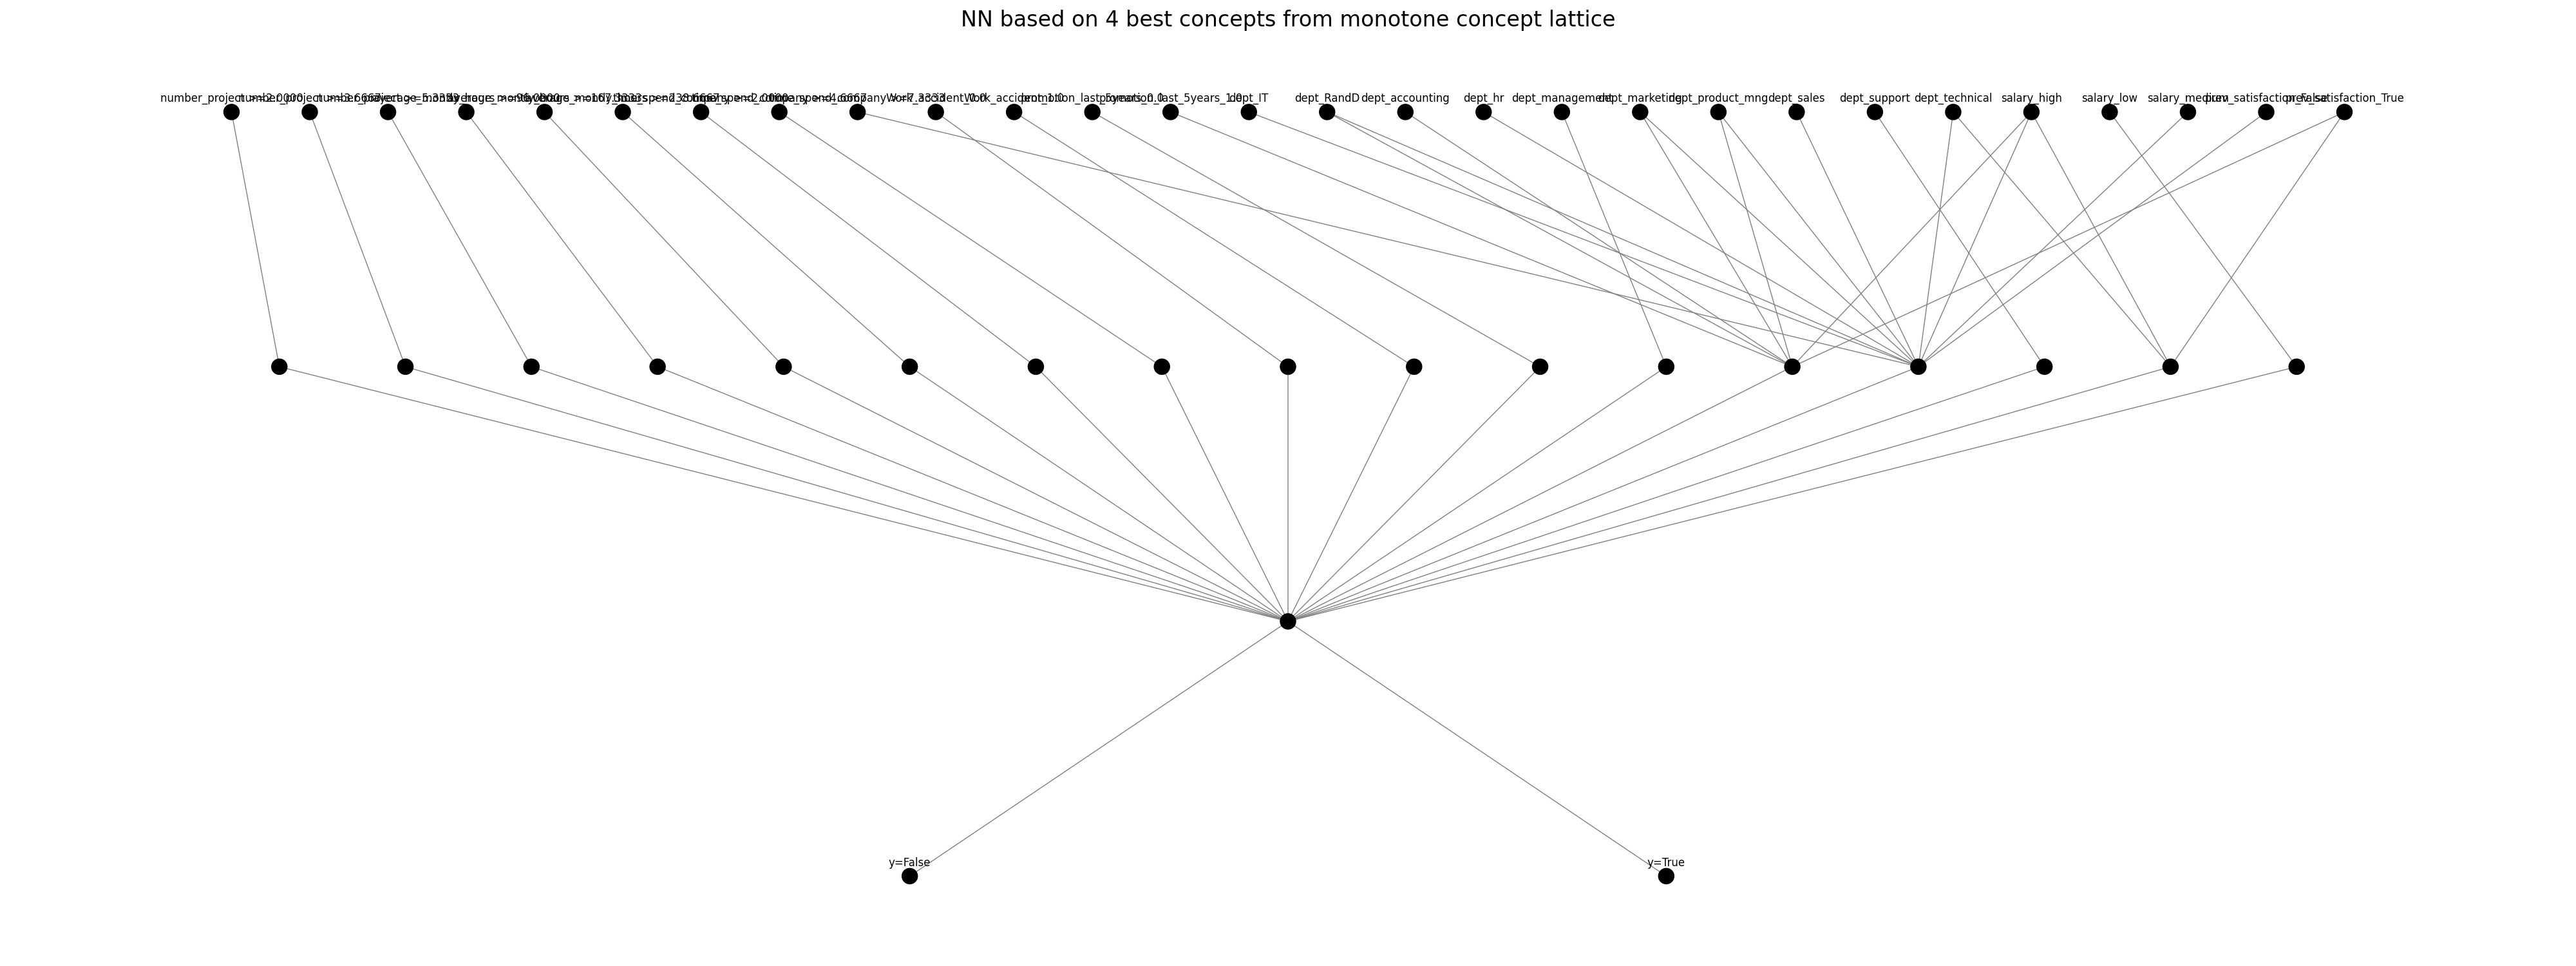
\includegraphics[width=\textwidth]{media/employees/NN_architecture_4concepts.png}
		\caption{NN architecture produced with the 4 best formal concepts(FCs) with interordinal encoding}
		\label{fig:4concepts-inter}
	\end{figure}
	
	The interordinal encoding works by applying both ordinal and inverse ordinal encoding at the same time. It preserves connections between values near the nodes, thus giving a notable performance boost to model performances while working with specific feature types such as age.
	
	\newpage
	
	\begin{figure}[h]
		\centering
		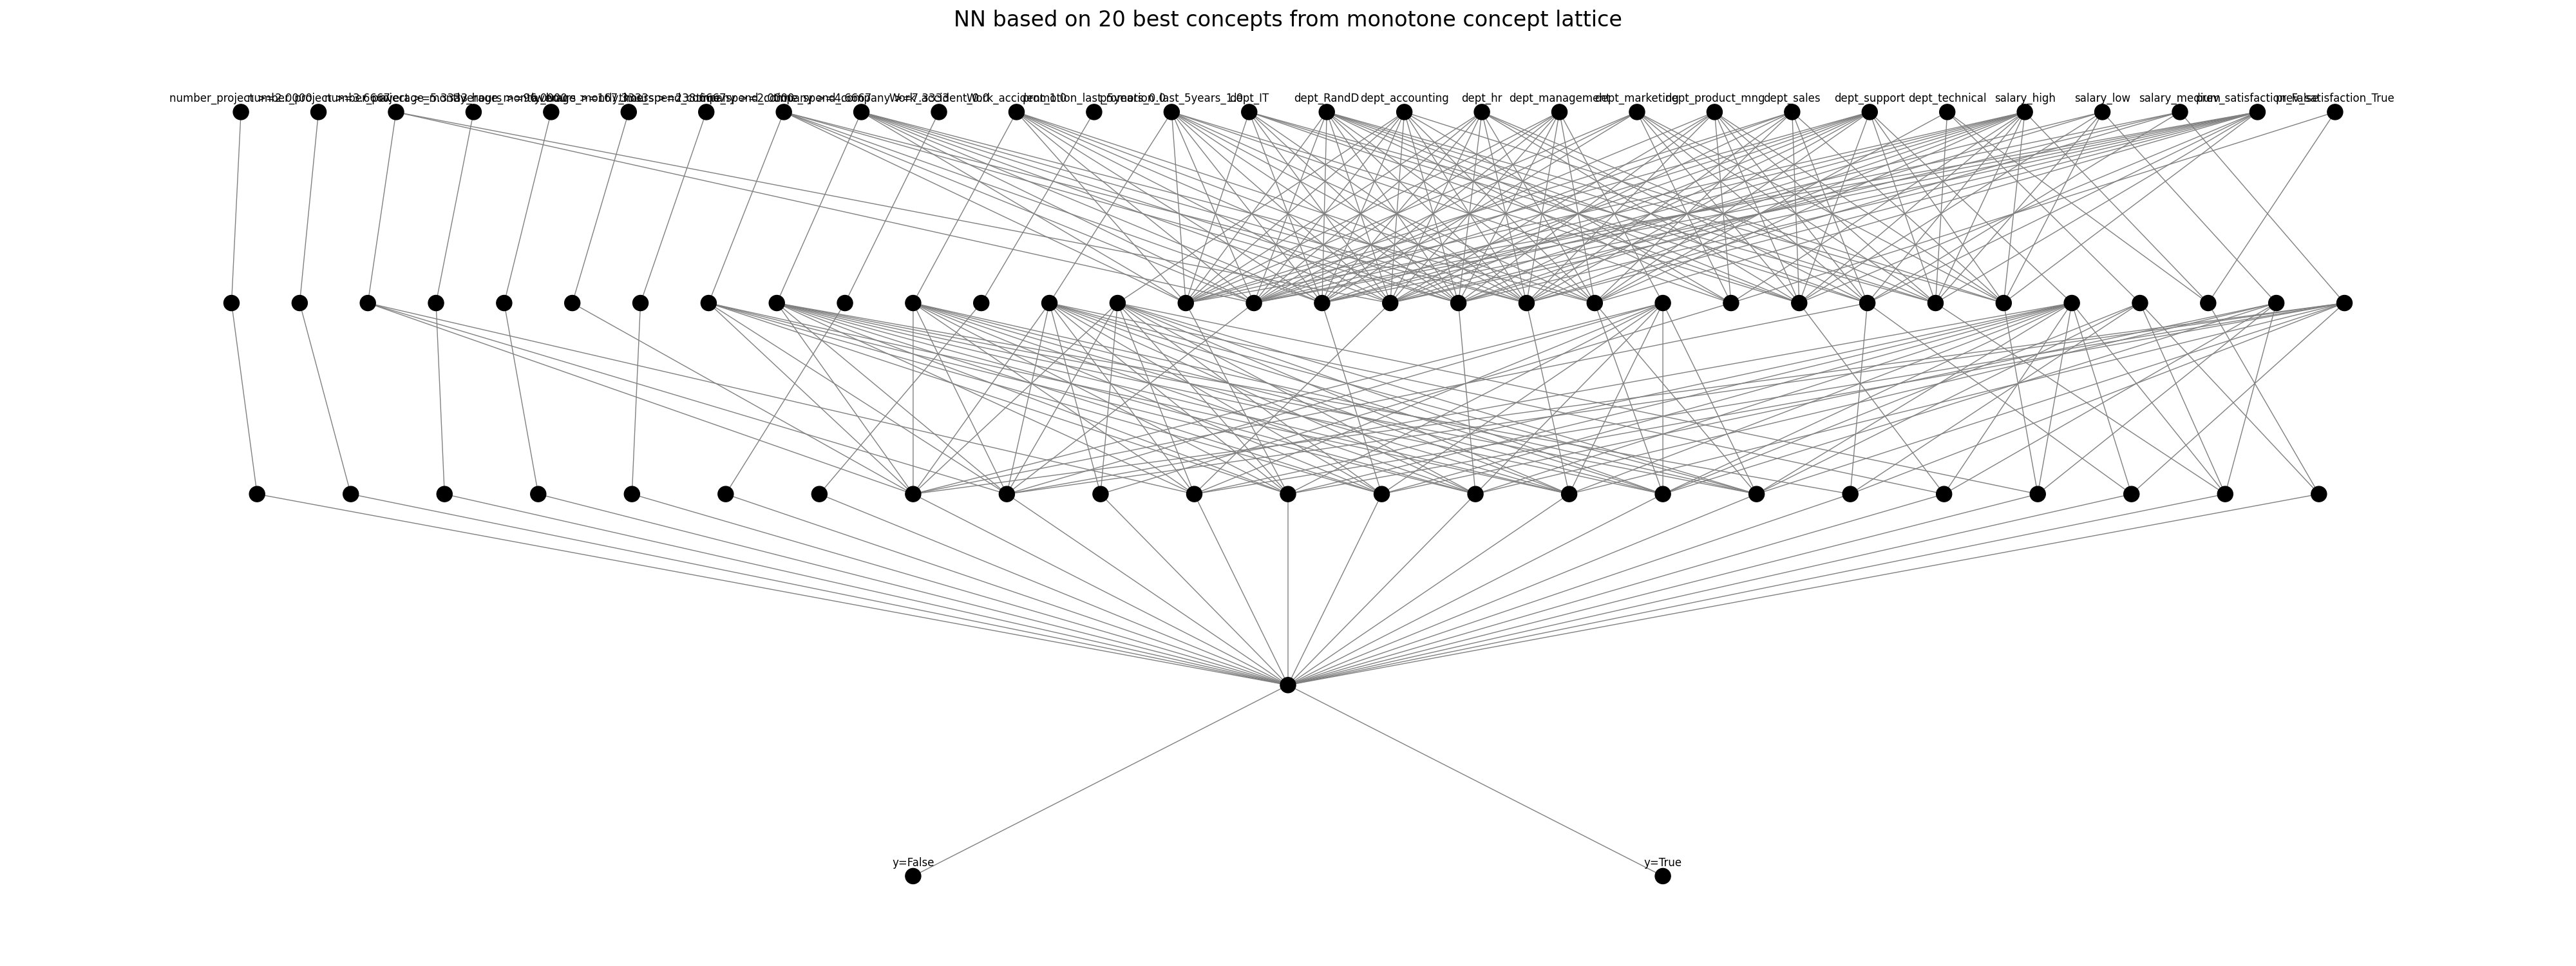
\includegraphics[width=\textwidth]{media/employees/NN_architecture_20concepts.png}
		\caption{NN architecture produced with the 20 best formal concepts(FCs) with interordinal encoding}
		\label{fig:20concepts-inter}
	\end{figure}
	
	 A finer numerical feature binarization should be considered in terms of its influence on the quality of predictions. With the increase in quantity of features, new dependencies in numerical data could be found. Table A.3 shows the performance metrics for this case; \figref{fig:4concepts-coarse} and \figref{fig:20concepts-coarse} demonstrate the NN architectures with this type of encoding.
	
	\begin{figure}[h]
		\centering
		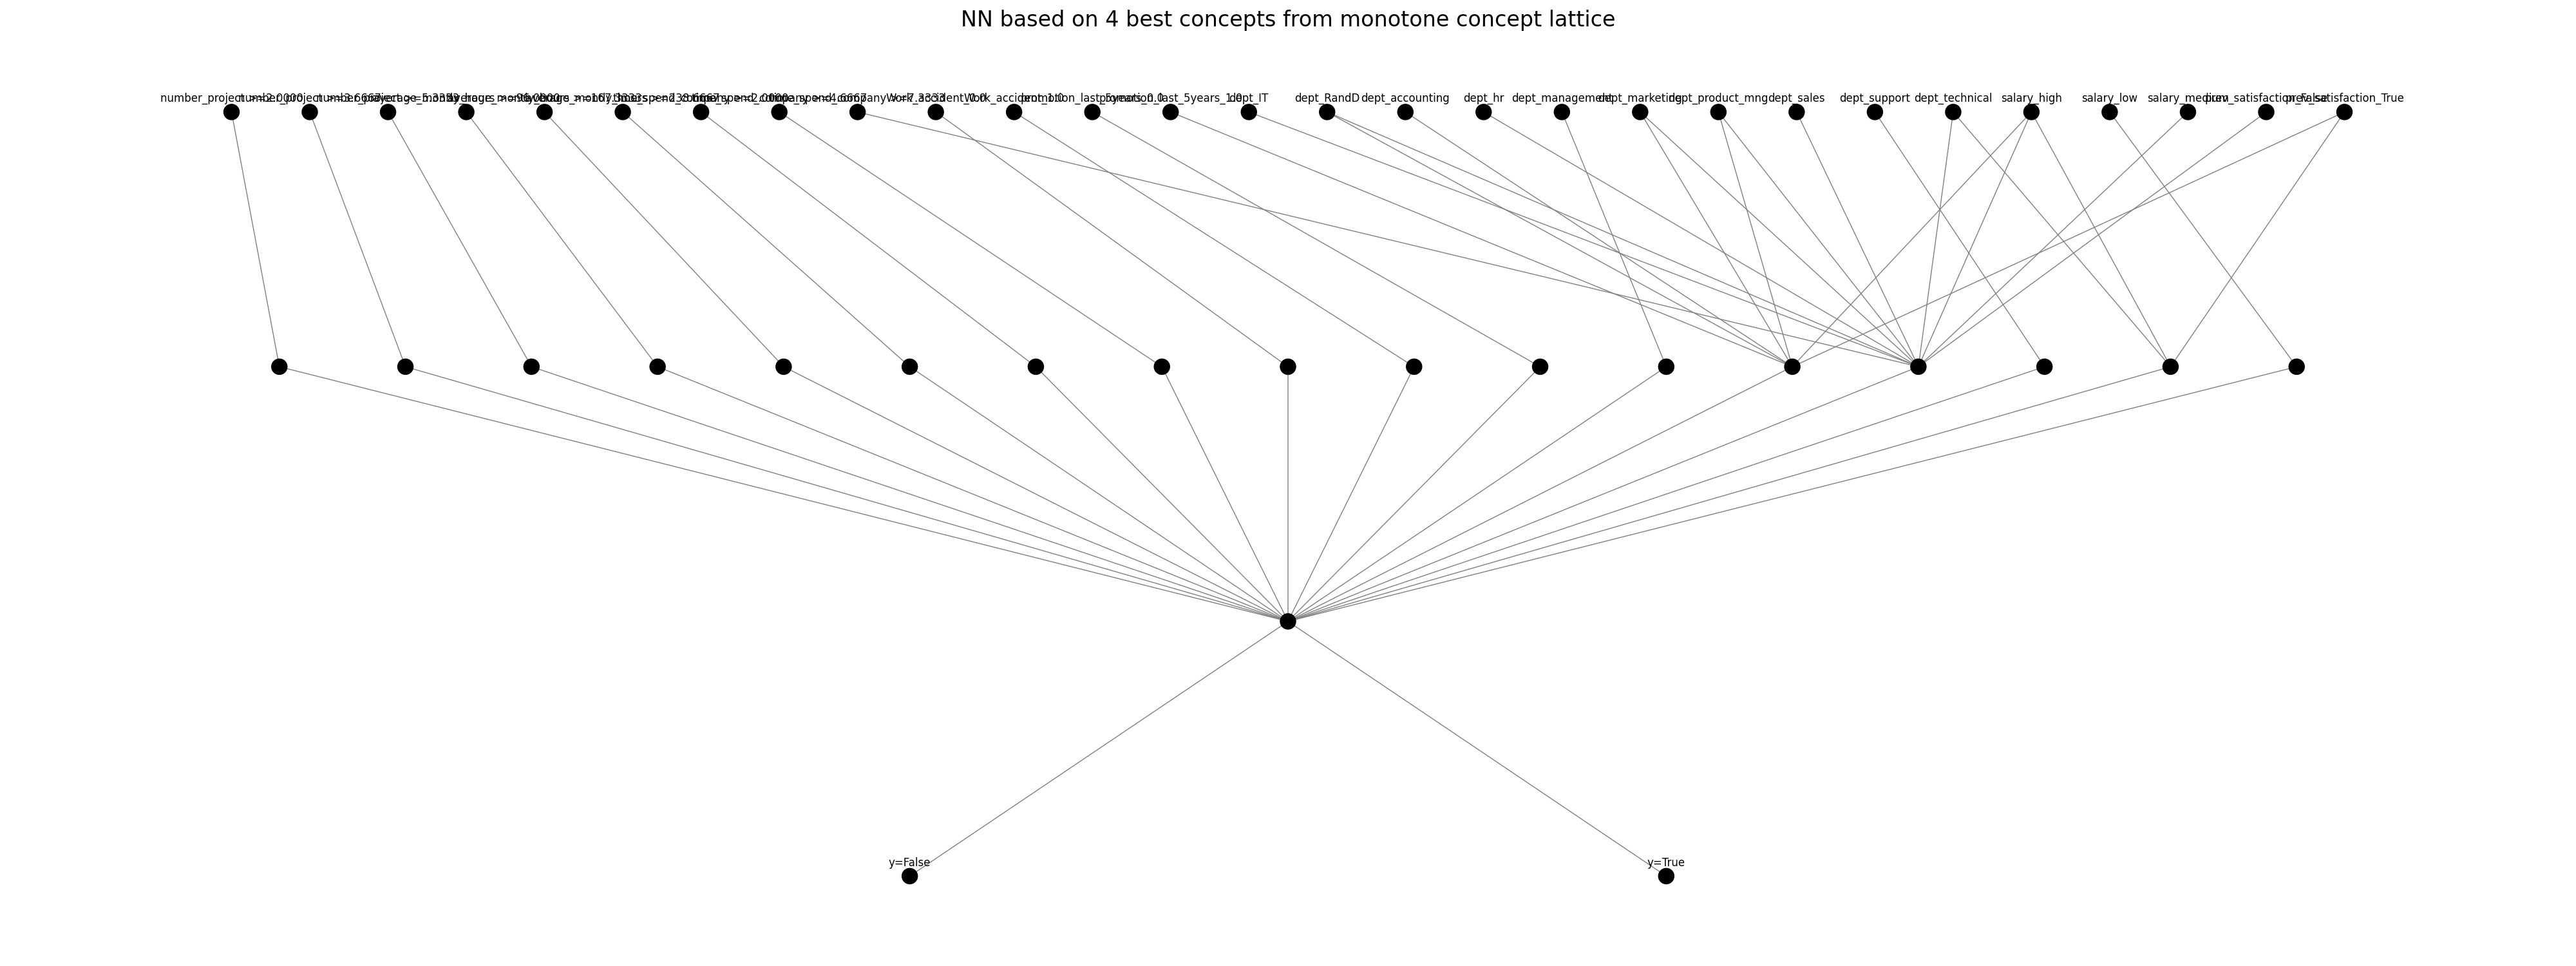
\includegraphics[width=\textwidth]{media/employees/NN_architecture_4concepts.png}
		\caption{NN architecture produced with the 4 best formal concepts(FCs) with finer ordinal encoding}
		\label{fig:4concepts-coarse}
	\end{figure}
	
	\newpage
	
	\begin{figure}[h]
		\centering
		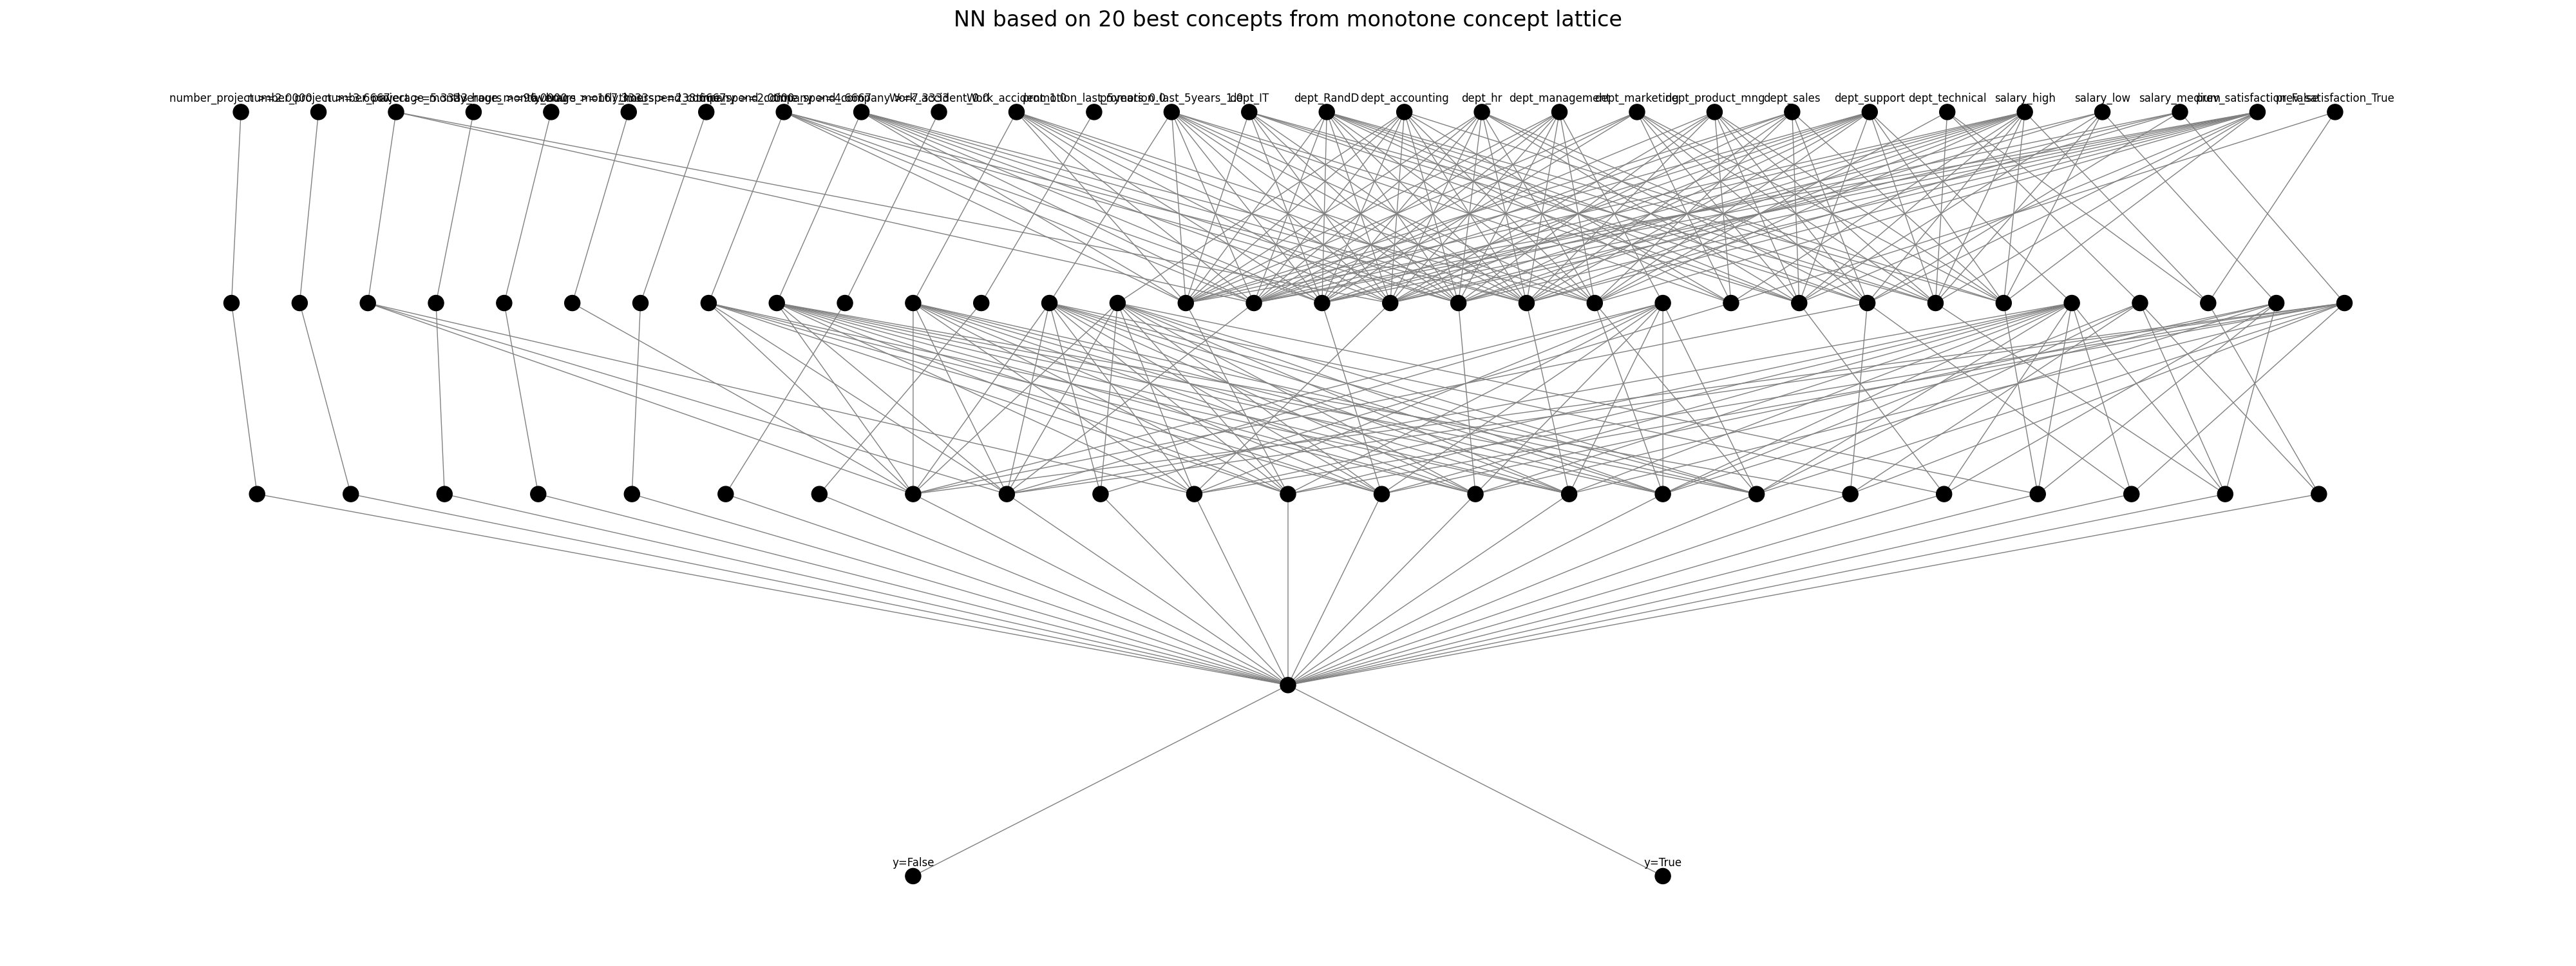
\includegraphics[width=\textwidth]{media/employees/NN_architecture_20concepts.png}
		\caption{NN architecture produced with the 20 best formal concepts(FCs) with finer ordinal encoding}
		\label{fig:20concepts-coarse}
	\end{figure}
	
	Finally, the impact of an increase in number formal concepts used to construct a concept lattice needs to be considered. Results of evaluating performance metrics on data with ordinal encoding of numerical features can be seen on \figref{fig:metrix}.  
	
	\begin{figure}[h]
		\centering
		\subfigure[]{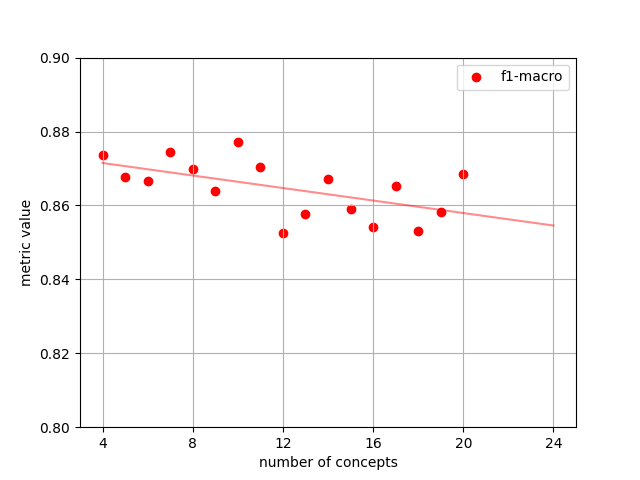
\includegraphics[width=0.45\textwidth]{media/employees/f1_score.png}}
		\subfigure[]{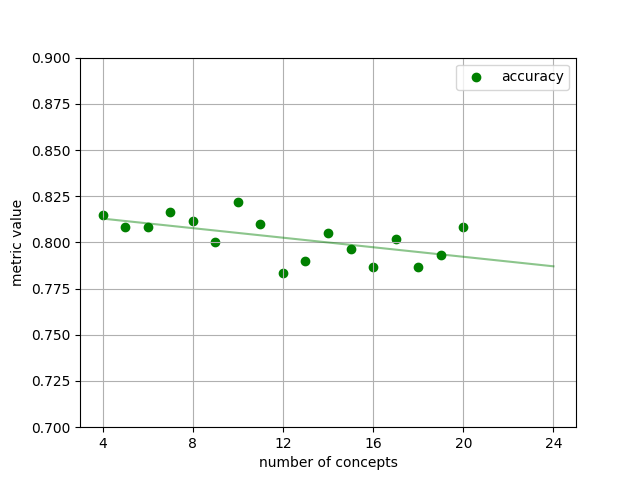
\includegraphics[width=0.45\textwidth]{media/employees/accuracy.png}}\\ 
		\caption{Model performance metrics as functions of number of concepts}
		\label{fig:metrix}
	\end{figure}
	
	\newpage
	
	\subsection{Model evaluation on the Estonia Disaster Passenger List dataset}
	
	This dataset small both in terms of number of features and objects and its only numerical feature is age. Therefore, interordinal encoding is the only logical choice for this case since it conserves closeness relation between people of similar age in different age groups. Here lattices from 21 concepts, which is minimal possible amount, and 25 concepts are considered, as shown in \figref{fig:21concepts} and \figref{fig:25concepts}, performance measures of those NNs can be seen in table A.4.
	
	\begin{figure}[h]
		\centering
		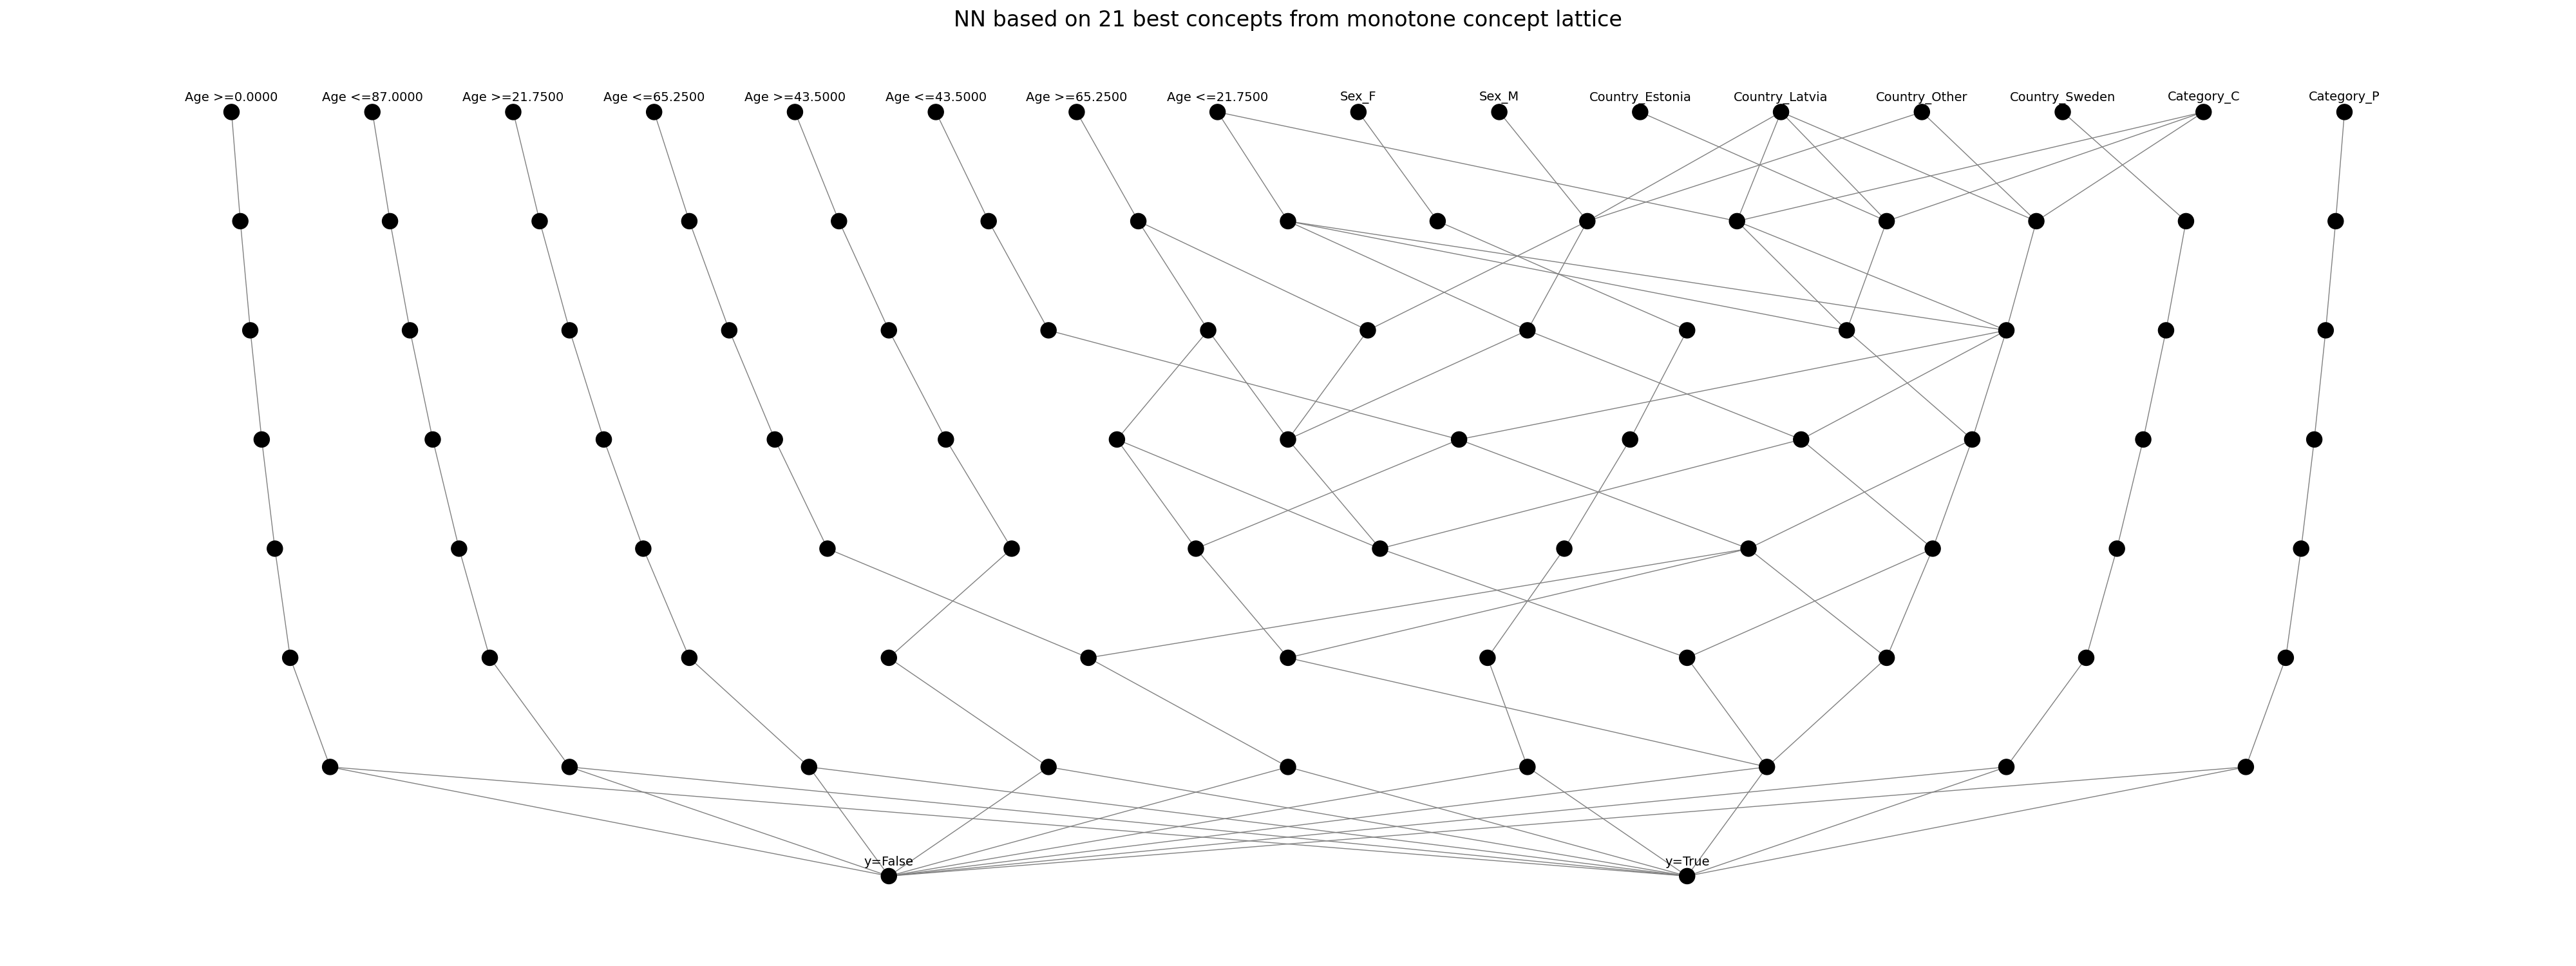
\includegraphics[width=\textwidth]{media/eesti/NN_architecture_21concepts.png}
		\caption{NN architecture produced with the 21 best formal concepts(FCs) on Estonia Disaster dataset}
		\label{fig:21concepts}
	\end{figure}
	
	\begin{figure}[h]
		\centering
		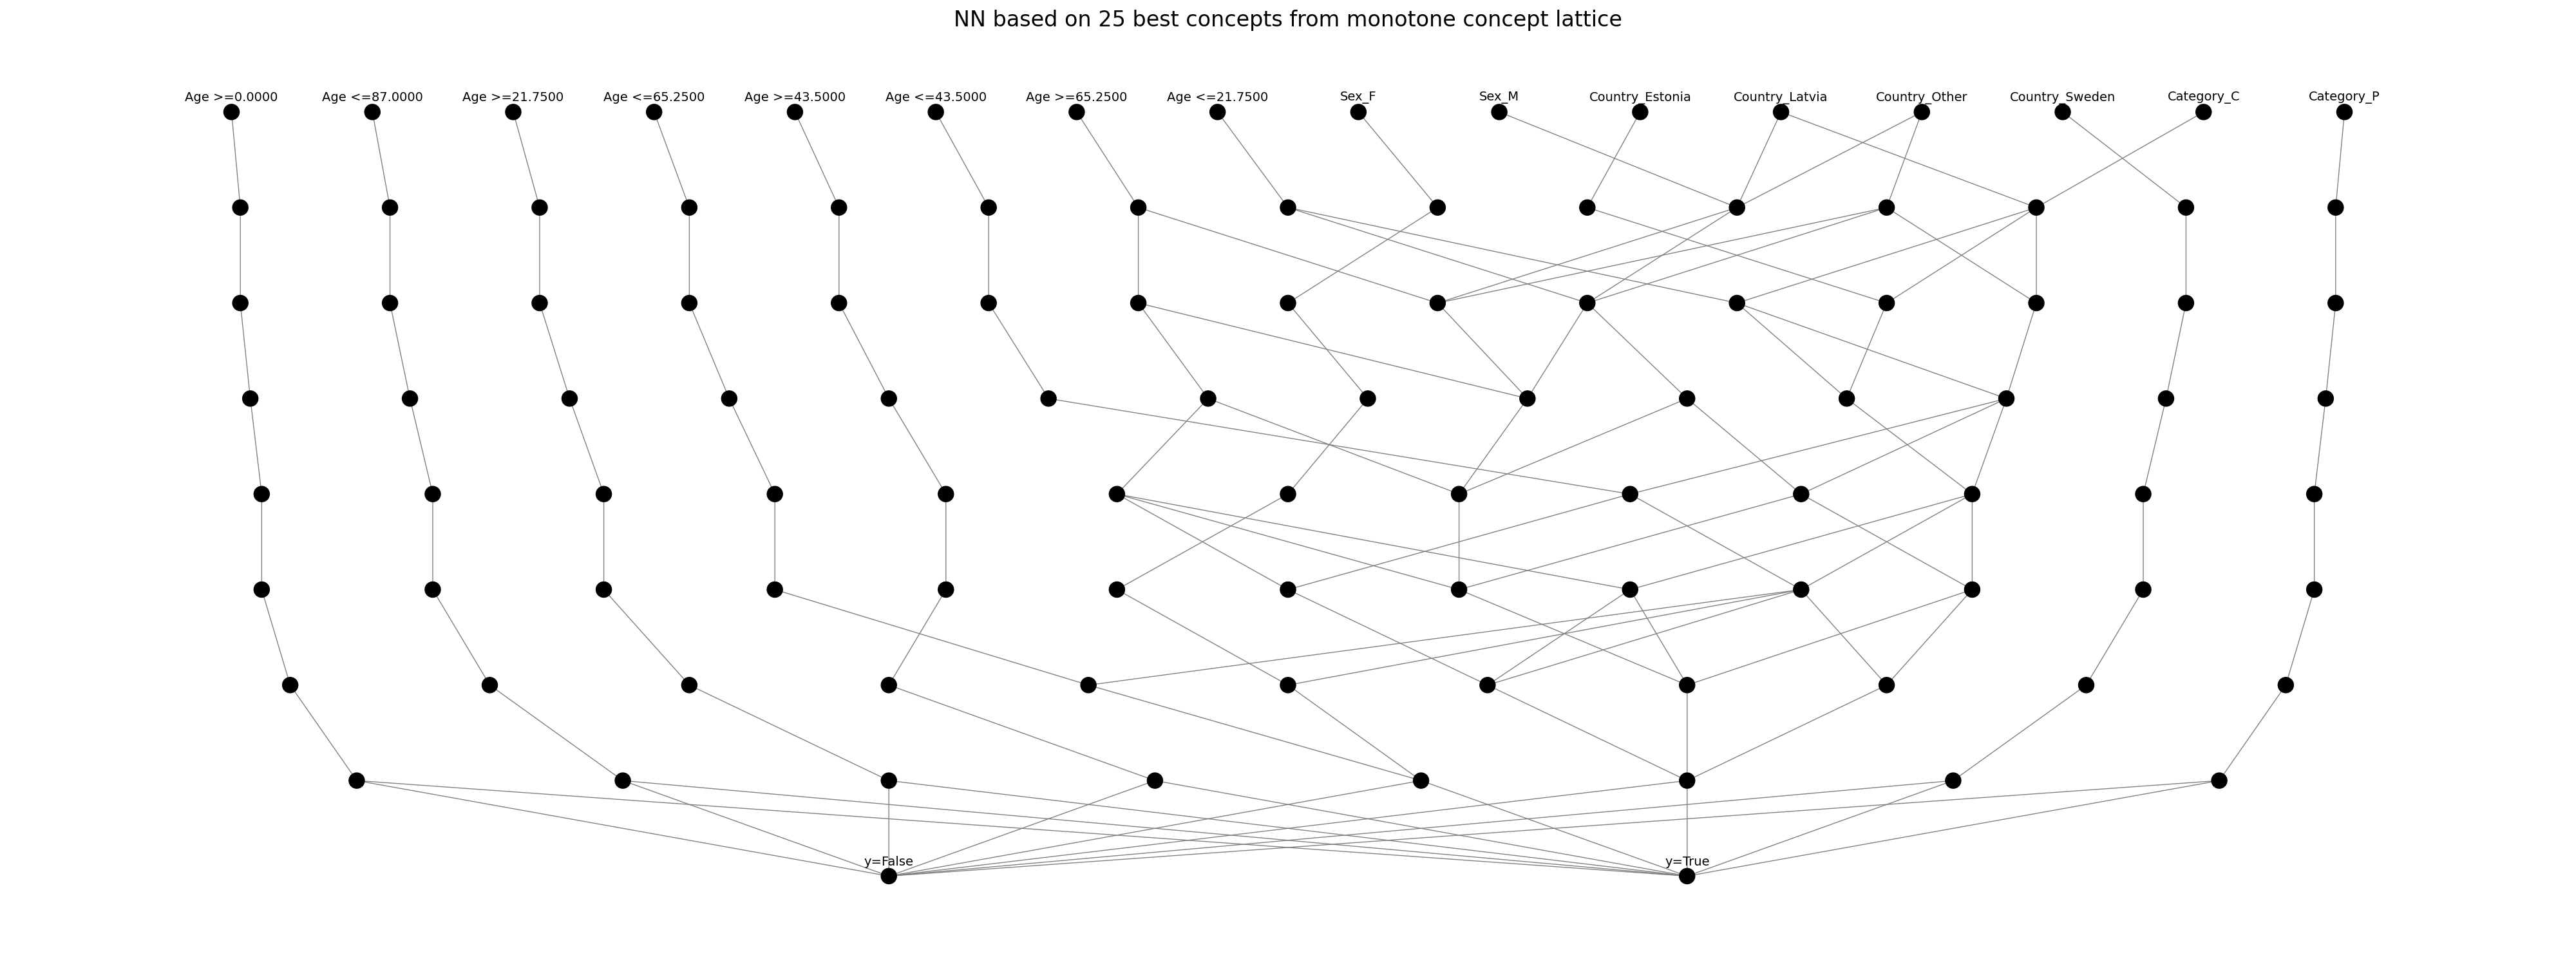
\includegraphics[width=\textwidth]{media/eesti/NN_architecture_25concepts.png}
		\caption{NN architecture produced with the 25 best formal concepts(FCs) on Estonia Disaster dataset}
		\label{fig:25concepts}
	\end{figure}
	
	\begin{results}
		
		Finer binarization produces better results in terms of model metrics than both the baseline and binarization using interordinal encoding with similar number of nodes, however this comes at the cost of interpretability. Increasing the number of formal concepts used to construct the concept lattice does not improve the model's performance; on the contrary, it seems to correlate with decrease in classification performance. Furthermore, the NN architecture used in this work struggles with overfitting on skewed data as exemplified by the Estonia Disaster dataset.
		
	\end{results}
	
	\section*{Conclusion}
	\addcontentsline{toc}{section}{\MakeUppercase{Conclusion}}
	
		Neural Networks based on concept lattices perform on par with several ensemble models and show promise in some machine learning applications. As exemplified by the Estonia Disaster dataset, these NNs can show connections between various features and their impact on its final decision, hence improving human interpretability of their inner workings.
		 
	
	\pagebreak
	\section*{Appendix A}
	\addcontentsline{toc}{section}{\MakeUppercase{Appendix A}}
	

	\begin{center}
		\noindent \textbf{Table A.1} Baseline NN performance on the Employee Attrition dataset 
		\begin{tblr}{width=.80\linewidth,
				colspec={|X[3,l]|X[c]|X[c]|}}
			\hline
			\textbf{Classifier} & \textbf{$f_1$-score} & \textbf{accuracy}\\
			\hline
			GaussianNB & 0.831797 & 0.756667\\
			\hline
			RandomForestClassifier & 0.888889 & 0.838333\\
			\hline
			HistGradientBoostingClassifier & 0.879147 & 0.830000\\
			\hline
			NeuralFCA(4 concepts) & 0.864310 & 0.801667\\
			\hline
			NeuralFCA(20 concepts) & 0.864253 & 0.800000\\
			\hline
		\end{tblr}
	\end{center}
	
	\begin{center}
		\noindent \textbf{Table A.2} NN performance on the Employee Attrition dataset with interordinal encoding
		\begin{tblr}{width=.80\linewidth,
				colspec={|X[3,l]|X[c]|X[c]|}}
			\hline
			\textbf{Classifier} & \textbf{$f_1$-score} & \textbf{accuracy}\\
			\hline
			GaussianNB & 0.831797 & 0.756667\\
			\hline
			RandomForestClassifier & 0.888889 & 0.838333\\
			\hline
			HistGradientBoostingClassifier & 0.879147 & 0.830000\\
			\hline
			NeuralFCA(4 concepts) & 0.870748 & 0.810000\\
			\hline
			NeuralFCA(20 concepts) & 0.856487 & 0.791667\\
			\hline
		\end{tblr}
	\end{center}
	
	\begin{center}
		\noindent \textbf{Table A.3} NN performance on the Employee Attrition dataset with finer ordinal encoding
		\begin{tblr}{width=.80\linewidth,
				colspec={|X[3,l]|X[c]|X[c]|}}
			\hline
			\textbf{Classifier} & \textbf{$f_1$-score} & \textbf{accuracy}\\
			\hline
			GaussianNB & 0.831797 & 0.756667\\
			\hline
			RandomForestClassifier & 0.888889 & 0.838333\\
			\hline
			HistGradientBoostingClassifier & 0.879147 & 0.830000\\
			\hline
			NeuralFCA(4 concepts) & 0.888889 & 0.838333\\
			\hline
			NeuralFCA(20 concepts) & 0.900115 & 0.855000\\
			\hline
		\end{tblr}
		\end{center}
	
	\newpage
	
	\begin{center}
		\noindent \textbf{Table A.4} NN performance on the Estonia disaster dataset
		\begin{tblr}{width=.80\linewidth,
				colspec={|X[3,l]|X[c]|X[c]|}}
			\hline
			\textbf{Classifier} & \textbf{$f_1$-score} & \textbf{accuracy}\\
			\hline
			GaussianNB & 0.831797 & 0.756667\\
			\hline
			RandomForestClassifier & 0.888889 & 0.838333\\
			\hline
			HistGradientBoostingClassifier & 0.879147 & 0.830000\\
			\hline
			NeuralFCA(21 concepts) & 0.00000 & 0.862903\\
			\hline
			NeuralFCA(25 concepts) & 0.000000 & 0.862903\\
			\hline
		\end{tblr}
	\end{center}
	
	\begin{thebibliography}{\kern\bibindent} \makeatletter \let\old@biblabel\@biblabel \def\@biblabel#1{\hspace{12.5 mm}\old@biblabel{#1}\kern\bibindent} \let\old@bibitem\bibitem \def\bibitem#1{\old@bibitem{#1}\leavevmode\kern-\bibindent} \makeatother
		
		\bibitem{NN_FCA}
		Kuznetsov, S.O., Makhazhanov, N., Ushakov, M. On Neural Network Architecture Based on Concept Lattices // Foundations of Intelligent Systems. ISMIS 2017. Lecture Notes in Computer Science(), vol 10352, pp. 653-663. Springer, Cham. https://doi.org/10.1007/978-3-319-60438-1\textunderscore64
	\end{thebibliography} 
\end{document}